% part_E: 원문 24--30쪽, VI. 평가 방법론 ~ IX. 결론 (참고문헌 제외)
\section{평가 방법론}

ASC 관련 지표를 논하기 전에, 먼저 기존 멀티미디어 통신에서 쓰여 온 품질 지표를 개관한다. 이미지와 비디오 전송에서는 PSNR과 구조적 유사도 지수(SSIM, structural similarity index measure)로 화소 수준과 구조 수준의 충실도를 평가해 왔다. 반면 학습된 지각적 이미지 패치 유사도(LPIPS, learned perceptual image patch similarity) [189]는 지각적 유사도를 더 잘 반영한다. 음성에서는 음성 품질의 지각적 평가(PESQ, perceptual evaluation of speech quality) [190]로 지각적 음성 품질을 측정할 수 있다. 그러나 이 지표들은 주로 수신 데이터의 복원 품질에 초점을 두므로 ASC에는 충분하지 않을 수 있다.

ASC의 지표는 세 가지 평가 범위로 정리할 수 있다. (i) 모달리티별 품질과 의미 충실도, (ii) 과업 수준·에이전트 수준의 효과성, (iii) 시스템 수준의 효율이다. 모달리티별 지표는 개별 표본이나 데이터 분포를 평가하고, 과업·에이전트 수준 지표는 한 에피소드나 에이전트 집단에 걸친 과업 결과를 측정하며, 시스템 수준 지표는 자원 소비와 효율을 나타낸다. 이 범위들은 평가 단위가 서로 다르므로 그 값을 직접 비교할 수 없다. 다중 모달 ASC라면 교차 모달 정렬(cross-modal alignment)도 고려할 수 있다. 표 X에 대표 지표의 평가 대상, 단위, 적용 범위를 정리했다.

\subsection{의도 중심 지표}

\paragraph{1) 모달리티별 지표:}
텍스트 전송에 관한 초기 연구는 BLEU(bilingual evaluation understudy)와 CIDEr(consensus-based image description evaluation) 지표를 사용했다. 그러나 이 지표들은 단어 수준이나 문자 수준의 일치만 포착하므로 의미의 일관성을 측정하기에는 부족하다. 이 한계를 해결하려고 맥락적 임베딩(contextual embedding) 기반 지표가 제안되었다. BERTScore [109]는 맥락적 토큰 임베딩 사이의 유사도를, MoverScore [191]는 맥락화된 표현 사이의 거리를 측정한다. BLEURT [192]와 COMET [193]은 사람의 판단과의 상관을 바탕으로 생성된 텍스트를 평가하는 데 쓸 수 있다. 또한 BARTScore [194]는 사전 학습된 시퀀스-투-시퀀스(sequence-to-sequence) 모델로 생성된 텍스트를 평가한다. 이 방법들은 $n$-그램 기반 지표와 달리 전송된 텍스트와 복원된 텍스트 사이의 의미 유사도를 고려한다.

PSNR과 SSIM 같은 기존 이미지 지표는 화소 수준이나 구조 수준의 정밀도를 평가하므로 의미 손실을 포착하는 데 한계가 있다. 의미 수준 평가를 위해, 의미 유사도 점수(SeSS, semantic similarity score) [195]는 객체 분할과 장면 그래프(scene graph)로 의미 충실도를 평가하고, 비전 트랜스포머 점수(ViTScore, vision Transformer score) [196]는 비전 트랜스포머가 추출한 표현을 비교한다. 비디오 데이터에서는 Fréchet 비디오 거리(FVD, Fréchet video distance) [197]가 시공간 표현의 분포 사이의 차이를 측정한다. 따라서 FVD는 개별 프레임이나 비디오 하나가 아니라 비디오 집합에 대해 평가해야 한다.

음성에서는 지각적 품질, 전사 정확도, 의미 보존이 서로 다른 평가 목표다. PESQ [190]는 지각적 음성 품질을 평가하고, WER과 CER은 전사 오류를 정량화한다. 그러나 전사 오류 지표는 의도한 의미가 보존되었더라도 표현이 다르면 불이익을 줄 수 있다. SpeechBERTScore [198]는 생성된 발화와 참조 발화의 자기 지도(self-supervised) 음성 표현을 비교하고, SeMaScore [199]는 음성 인식(ASR) 평가를 위해 인식 오류율과 의미 유사도를 결합한다. 따라서 이 지표들은 평가 대상이 지각적 음성 품질인지, 음성 표현의 유사도인지, 인식된 내용의 의미 정확도인지에 따라 골라야 한다.

이미지, 텍스트, 음성 외에도 ASC는 3D 점군(point cloud)과 시계열 센서 데이터를 다룰 수 있다. 점군의 충실도는 Chamfer 거리 [200] 같은 기하 지표로 평가할 수 있고, 시계열 복원은 RMSE나 동적 시간 워핑(DTW, dynamic time warping)으로 평가할 수 있다. 이 지표들은 과업 효과성이 아니라 기하적·시간적 충실도를 나타내므로, 관련이 있다면 하위 과업 성능을 따로 평가해야 한다.

\paragraph{2) 다중 모달 지표:}
다중 모달 ASC는 모달리티별 품질, 교차 모달 정렬, 하위 과업 성능의 관점에서 평가할 수 있다. 모달리티별 지표는 복원된 각 신호의 품질을 평가하고, 교차 모달 지표는 서로 다른 모달리티가 일관된 의미 내용을 보존하는지 평가한다. CLIPScore [201]는 이미지-텍스트 대응을 평가하고, CLAP 기반 유사도 [202]는 오디오-텍스트 정렬을 평가하는 데 쓸 수 있다. ImageBind [203]는 여러 모달리티에 걸친 공유 표현 공간을 제공하며, 이 공간에서 코사인 유사도나 Recall@K 같은 검색 기반 지표로 교차 모달 정렬을 측정할 수 있다.

그러나 교차 모달 유사도가 높다고 해서 과업과 관련된 정보가 보존되거나 과업이 성공적으로 수행된다는 보장은 없다. 예를 들어 한 모달리티에서 과업과 관련된 정보가 빠지더라도, 복원된 모달리티들은 공통 임베딩 공간에서 여전히 가까울 수 있다. 따라서 교차 모달 정렬은 모달리티별 품질, 그리고 검색 정확도, 객체 검출 성능, 과업 성공 확률 같은 하위 과업 성능과 함께 고려해야 한다.

\paragraph{3) 유사도 지표:}
생성된 기호의 표현력을 평가하려고 기호 사이의 유사도를 나타내는 지표가 쓰여 왔다. 지형 유사도(TopSim, topographic similarity) [204]는 비슷한 의미일수록 메시지도 더 비슷하게 배치되는지를 측정한다. 이 지표는 단순한 정확도보다는 구성성(compositionality)과 관련된다. 직관적으로 TopSim은 의미 공간에서의 쌍별 거리와 메시지 공간에서의 쌍별 거리 사이의 상관이다. 예를 들어 ``빨간 원''과 ``빨간 사각형''은 기호 하나만 다른 메시지에 대응하고, ``파란 삼각형''은 상당히 다른 메시지에 대응할 수 있다. 이런 대응은 TopSim이 높으며, 비슷한 의미가 비슷한 메시지로 표현되는 경향을 나타낸다. 다만 구조적 정렬이 성능 향상으로 이어지는지 확인하려면 TopSim 값을 하위 과업 정확도와 함께 사용해야 한다. NeSy에 기반한 최근의 창발적 의미 통신 연구 [38]는 두 상태 기술 $x$와 $y$ 사이의 의미적 겹침 정도를 정량화하는 의미 유사도 지표를 제안했다. 이 지표는 두 표현이 생성하는 의미 공간의 유사도를 측정한다. 값이 클수록 의미가 더 비슷하고, 작을수록 관련성이 낮음을 뜻한다.

KG를 사용한다면 개념 노드 사이의 평균 최소 경로 길이로 의미 유사도를 평가할 수 있다 [205]. 노드의 정보량(예: 개념의 확률)을 반영하면 사람의 직관을 포착하는 능력을 더 높일 수 있다. 따라서 노드/링크 기반 지표는 의미 오류 정정이나 텍스트 분석처럼 맥락을 정확히 인식하는 추론이 필요한 과업에 적합하다.

\paragraph{4) 추론 지표:}
BLEU, CIDEr, BERTScore 같은 이전 지표는 두 텍스트 입력을 수학적으로 비교해 점수를 계산했다. 이런 방식에서는 과업 목표를 이해하지 않은 채 점수가 계산된다. 반면 LLM-as-a-Judge [206]는 LLM을 평가자로 써서 인지적 평가의 새로운 가능성을 제시한다. 이 평가 방법은 [207]에서 통신 시스템 안에서 AI가 생성한 응답의 품질을 평가하는 데 구현되었다. 구체적으로, 이 방법은 상세한 피드백을 제공하고 과업에 따라 평가 기준을 조정하는 중재 계층 역할을 한다.

추론 능력은 수신기가 송신기에 보내는 질의 횟수와 의미 표현의 효율을 결합한 통신 대칭 지수(communication symmetry index)로 계산한다 [17]. 또한 [83]에서는 전문가가 생성한 경로와 모델이 생성한 경로 사이의 유사도를 측정하는 경로 추론 정확도(path reasoning accuracy)를 암묵적 의미를 추론하는 능력의 척도로 사용한다.

LLM-as-a-Judge는 목표 지향 대화나 다단계 과업 계획처럼 정답 레이블이 없는 개방형 의도 평가에 특히 적합하다. 그러나 계산 비용 때문에 실시간 ASC 평가에는 실용적이지 않으며, 이런 경우에는 경로 추론 정확도가 가벼운 대안이 된다.

\paragraph{5) 설명 가능성 지표:}
설명 가능한 AI(XAI, explainable AI) 기법은 ASC 에이전트가 특정한 통신 결정을 내리는 이유를 살펴보는 실용적인 해법이 될 수 있다 [208]. 예를 들어 SHAP [209]과 Grad-CAM [210] 같은 기여도 분석(attribution) 방법은 입력 특징에 중요도 점수를 부여한다. 이 방법들을 ASC에 적용하면, 관측의 어느 부분이 전송할 의미 토큰의 선택을 이끄는지, 또는 시스템 1/시스템 2 전환을 촉발하는지 드러낼 수 있다. 개념 활성화 벡터 검정(TCAV, testing with concept activation vectors) [211] 같은 개념 기반 방법은 학습된 의미 표현이 사람이 해석할 수 있는 개념에 대응하는지 살펴보는 데 쓸 수 있다. XAI 문헌은 설명 자체를 평가하는 기준도 제공한다. 충실성(faithfulness; 예컨대 삭제/삽입 검사로 확인하는, 설명이 실제 모델 동작을 반영하는지 여부), 강건성(robustness; 비슷한 입력이 비슷한 설명을 낳는지 여부), 복잡도(complexity; 설명이 해석할 수 있을 만큼 희소한지 여부)가 그 예다 [212]. ASC에서는 이 지표들로 토큰 선택이나 전송 생략 같은 자율적 전송 결정을 분석할 수 있다.

\subsection{에이전트 중심 지표}

에이전트형 시스템의 성능을 평가하려면, 비트 오류율(BER)과 지연에 관한 전통적 지표 외에 과업 수행의 효율을 정량화하는 지표가 필요하다. 과업 성공 확률(TSP, task success probability) [61]은 주어진 과업이 의도한 목표를 달성하는 비율을 나타낸다. TSP는 응용의 성공 여부로 평가하므로 과업별 성능을 추론할 수는 있지만, 일반화에는 여전히 제약이 있다. 과업 지향 왜곡(ToD, task-oriented distortion) [213]은 과업 특성에 따른 출력 품질 저하의 정도를 나타낸다. 종단 간 지연 대 과업 보상 곡선 [214]은 시스템 전체의 지연과 과업 성능 사이의 상충 관계를 정량화한다. 더 나아가 다차원 에이전트-과업 효용(agent-task utility)은 에이전트형 응용이 사용자 경험과 과업 수행 효율을 얼마나 높이는지 평가한다 [215]. 이 지표는 명확성, 완전성, 효율을 포함한 여러 성능 차원을 포착해 기존 종단 간 성공 지표의 한계를 극복한다. TSP는 분류나 내비게이션처럼 목표 달성 여부가 이산적인 과업에 권장되는 반면, ToD는 부분적 품질 저하가 의미를 지니는 연속 출력 과업(예: 분할 과업)에 더 적합하다. 지연 대 과업 보상 곡선은 실시간 제약 아래에서 시스템 수준의 상충 관계를 포착하도록 평가해야 한다. 네트워크 관리, 자원 할당, 이상 탐지 같은 과업에 걸쳐 LLM 기반 에이전트를 다차원으로 평가하는 데에는 에이전트-과업 효용이 알맞은 평가 지표다. 실제로는 이 지표들에도 한계가 있다. TSP와 ToD는 과업별 정답(ground truth)이 필요해 이질적인 과업 전반에 적용하기 어렵다. 지연-보상 곡선은 배포 환경에 따라 달라지고, LLM 기반 효용 점수는 평가자 모델의 선택에 따라 달라진다.

\subsection{시스템 효율 지표}

\paragraph{1) 계산 복잡도:}
에이전트의 계산 효율은 모델 크기와 추론 비용으로 평가할 수 있다. 흔히 쓰는 지표로는 파라미터 수, 그리고 추론에 필요한 초당 부동소수점 연산(FLOP) 수나 곱셈-누산(multiply--accumulate) 연산 수가 있다 [174], [216]. 엣지 환경에서는, 특히 계획이나 자기 성찰(self-reflection) 과정이 있을 때 메모리 사용량과 결정당 에너지 소비를 쓸 수 있다 [174]. 또한 응답 지연은 첫 토큰까지의 시간(TTFT, time-to-first-token)과 토큰 간 시간(TBT, time-between-tokens)으로 측정할 수 있으며, 이 값들은 하드웨어 가속기 활용도를 반영한다 [216]. 토큰 수는 LLM 사용량을 측정하는 데 쓰이며 [75], 전환 사이의 평균 토큰 수를 기준으로 시스템 1에서 시스템 2로 전환하는 지연을 나타내는 지표로도 쓰인다 [217]. 이 지표로 가벼운 추론(inference)과 무거운 추론(reasoning) 사이를 동적으로 전환하는 에이전트를 평가할 수 있다.

\paragraph{2) 통신 오버헤드:}
분산 구조나 엣지-클라우드 구조에서는 에이전트 간 상호작용이 통신 오버헤드를 낳는다. 대표적 평가 지표는 갱신당 통신량과 협력 라운드당 전송 데이터량이다 [174], [216]. 다중 에이전트 시스템에서는 에이전트가 관측이나 중간 활성값을 교환할 때 대역폭 소비와 패킷 전달률을 측정한다. 차세대 무선 네트워크에서는 지능형 제어로 불필요한 전송을 줄이는 것도 통신 효율의 지표로 여긴다 [218].

\paragraph{3) 시스템 수준 효율:}
처리량, 종단 간 지연, 스펙트럼 효율, 에너지 효율 같은 시스템 수준 지표는 의미 통신에도 여전히 적용된다. ASC에서 이 지표들은 주어진 의미 성능이나 과업 성능을 달성하는 데 필요한 시스템 자원을 정량화한다. 따라서 자원 소비를 그에 대응하는 의미 성능이나 과업 성능과 함께 평가할 수 있다.

효과성 정규화 지표(effectiveness-normalized metric)는 과업 성능을 그에 대응하는 자원 비용과 연결하는 한 가지 방법이다. 대표적인 예로 전송 비트당 또는 채널 사용당 과업 효용, 줄당 성공 과업 수, 초당 성공 과업 수, 단위 대역폭당 과업 효용이 있다. 역수 형태는 다른 양을 나타내므로 지표의 방향과 단위를 명시해야 한다. 에너지의 경우, 줄당 완료 과업 수나 과업 효용은 에너지 효율을 측정하고, 과업당 줄로 나타내는 완료 과업당 에너지는 그에 대응하는 비용을 측정한다. 시간에도 같은 구분이 적용된다. 종단 간 지연은 시간 비용을 측정하고, 초당 성공 과업 수는 시간으로 정규화한 효과성을 측정한다.

의미 전송을 반영하기 위해, 초당 전달되는 의미 정보의 양을 의미 단위(suts/s)로 정량화하는 의미 전송률(semantic rate)과, 의미 전송률을 점유 대역폭으로 정규화한 의미 스펙트럼 효율(suts/s/Hz)이 도입되었다 [219]. 이 지표들은 특정 원천과 과업에 대해 의미 단위가 명시적으로 정의될 때 유용하다. 그러나 텍스트 통신에서 정의한 의미 단위가 음성, 시각, 점군, 다중 모달 표현에서 정의한 의미 단위와 반드시 같지는 않다. 따라서 의미 전송률은 ASC의 보편적 척도가 아니라 모달리티별·과업별 지표로 해석해야 한다.

공통 의미 단위가 없으면 같은 하위 과업과 성능 지표를 기준으로 시스템을 비교할 수 있다. 지연과 에너지를 평가할 때는 시스템 경계도 정의해야 한다. 예를 들어 평가 범위에 송신기만 넣을 수도 있고, 송신기와 수신기를 넣을 수도 있으며, 기기-엣지-클라우드 시스템 전체를 넣을 수도 있다. 서로 다른 시스템 경계에서 얻은 지연과 에너지 결과는 직접 비교할 수 없을 수 있다.

\subsection{벤치마크 데이터셋}

LLM이 발전하면서 LLM 기반 에이전트의 추론, 의사 결정, 상호작용 능력을 평가하는 벤치마크 데이터셋이 많이 제안되었다. 시퀀스 예측이나 지각에 초점을 둔 자연어 처리(NLP)·시각 벤치마크와 달리, 이 새로운 벤치마크들은 에이전트 수준의 지능과 상호작용 행동을 평가하도록 설계되었다. 표 XI에 일반 LLM 기반 에이전트를 평가하는 벤치마크와 통신 환경에서 에이전트 성능을 평가하는 벤치마크를 정리했다.

에이전트형 시스템을 위한 벤치마크 데이터셋이 활발히 제안되어 왔지만, 가상 현실(VR, virtual reality), 증강 현실(AR, augmented reality), UAV 군집 시나리오에서 지능형 통신을 평가하기에는 아직 한계가 있다. 따라서 앞으로의 통신 연구에서는 의미 잡음에 대한 복원력, 지식의 진화, 이질적 에이전트형 통신을 평가하는 벤치마크 데이터셋을 개발하고 적용해야 한다.

\setcounter{table}{10}
\begin{table}[htbp]
\centering
\caption{ASC 관련 벤치마크 요약}
\label{tab:11}
\footnotesize
\renewcommand{\arraystretch}{1.25}
\begin{tabularx}{\linewidth}{|>{\centering\arraybackslash}p{1.7cm}|>{\centering\arraybackslash}p{2.7cm}|>{\centering\arraybackslash}p{2.0cm}|>{\centering\arraybackslash}X|>{\centering\arraybackslash}X|}
\hline
\textbf{분야} & \textbf{벤치마크} & \textbf{영역} & \textbf{과업} & \textbf{주요 특징} \\
\hline
\multirow{3}{=}{\centering 일반 LLM 에이전트}
 & AgentBench [220] & LLM 에이전트 평가 & 단일 에이전트 추론, 도구 사용, 적응적 의사 결정 & 에이전트 수준의 과업 지향 지능을 평가하는 표준 기준을 제공 \\
\cline{2-5}
 & MultiAgentBench [221] & 다중 에이전트 시스템 & 협력/경쟁 과업 (예: 협상, 자원 할당, 계획 등) & 다중 에이전트 환경에서 창발적 통신과 조정 효율을 평가 \\
\cline{2-5}
 & SwarmBench [222] & 군집 지능 & 국소 정보에 기반한 다중 에이전트 협력 & 중앙 제어가 없는 격자 환경. 창발적 조정 전략을 평가 \\
\hline
\multirow{6}{=}{\centering 무선 통신}
 & TeleQnA [223] & 질의응답(QA) & 일반 통신 분야 QA & 자동 생성 후 사람이 검증 \\
\cline{2-5}
 & TeleMath [224] & 수학 & 통신 분야의 수치 문제 풀이 & 신호 처리, 네트워크 최적화, 성능 분석을 포괄 \\
\cline{2-5}
 & ORAN-Bench [225] & O-RAN & O-RAN 규격 지식 평가 & 이상 탐지, 네트워크 분석, 코드 생성 과업을 포함 \\
\cline{2-5}
 & WirelessAgent [226] & 무선 네트워크 관리 & 네트워크 슬라이싱 관리 & LLM 기반 에이전트가 복잡한 무선 과업을 관리할 수 있음을 보임 \\
\cline{2-5}
 & 5G-NIDD [227] & 네트워크 보안 & 5G 네트워크 침입 탐지 & 실제 5G 테스트베드로 구축한, 레이블이 모두 달린 데이터셋 \\
\cline{2-5}
 & TSpec-LLM [228] & 3GPP 규격 평가 & 3GPP 문서 전체 & 통신 표준에 대한 LLM 사전 학습과 미세 조정을 위한 공개 데이터셋 \\
\hline
\end{tabularx}
\end{table}

\section{유망한 응용과 활용 사례}

ASC는 다양한 6G 서비스에 적용될 수 있으며, 아래 활용 사례들은 서로 다른 ASC 적용 환경을 대표한다. 이 응용들에서는 과업 성능이 통신에 좌우되며, 자율적이고 과업을 인식하는 정보 교환이 필요하다. NTN에서는 동적인 채널 조건과 긴 전파 지연 아래에서 예측과 자원을 고려한 정보 교환이 필요하다. 자율주행차에는 여러 에이전트 사이의 저지연·고신뢰 조정이 필요하고, 디지털 트윈에는 물리 개체와 사이버 개체 사이의 지속적인 의미 상태 동기화가 필요하다. 따라서 세 사례는 V절에서 논한 예측과 적응, 다중 에이전트 조정, 의미 상태 동기화를 각각 보여 준다.

\subsection{비지상 네트워크}

비지상 네트워크(NTN)는 음영 지역까지 통신 커버리지를 넓히는 핵심 기반 기술로 여겨진다 [229]. 그럼에도 NTN에는 높은 지연, 위성의 빠른 이동, 제한된 자원 같은 기술적 과제가 있다. 이런 요구를 충족하려면 효율적인 통신과 자율적인 네트워크 관리 메커니즘이 필요하다. 이런 맥락에서 TOSC와 자율 에이전트의 결합이 설계 대안으로 떠오르고 있다 [230]. 최근 연구들은 UAV [231]--[233]와 위성 [234]--[236] 같은 비지상 플랫폼을 위한 ASC를 연구했다.

UAV 네트워크에서는 UAV 중계를 통한 효율적인 통신 구조를 제시하려고 확률적 의미 통신(PSC, probabilistic SC) 시스템 [231]이 개발되었다. RALLY(role-adaptive LLM-driven yoked) 내비게이션 프레임워크 [232]는 LLM 기반 의미 추론을 활용해 협력적 의사 결정을 가능하게 한다. 연합 MARL 프레임워크 [233]는 VAE로 강화한 비동기 연합 학습과 GNN 기반 다중 에이전트 DRL을 통합한다. 이 프레임워크는 초고신뢰 저지연 통신(URLLC, ultra-reliable low-latency communications) 기반 의미 통신에서 과업 성능, 에너지 효율, 커버리지, 부하 분산을 함께 최적화한다.

위성 네트워크에서는 RAG를 활용한 LLM 강화 모델링이 시스템 설계를 자동화하고, 전문가 혼합(mixture of experts) 방법으로 자원 할당을 지원한다 [234]. GSC 시스템은 위성 메가 군집(mega-constellation)을 위한 혁신적인 접근법이다 [235]. 이 시스템은 이산 시간 그래프 모델링으로 의미 부호기·복호기 배치 방법과 GSC 호환 라우팅 방법을 개발한다. LEO 위성 네트워크에서는 인지적 의미 증강(cognitive semantic augmentation)이 이산 과업 지향 JSCC와 의미 증강을 결합해 효율적인 다중 스펙트럼 이미지 전송을 가능하게 한다 [236].

NTN 기반 ASC의 실현 가능성은 엄격한 에너지·처리 제약 때문에 컴퓨팅 배치에 좌우된다. 또한 지연이 큰 링크로 세계 모델이나 규약을 동기화하면 오버헤드가 크다. 실제 배포에서는 지상 부문이 비용이 큰 추론을 맡고, 위성 탑재 에이전트는 저수준 동작으로 제한해야 한다. NTN에서 ASC의 잠재력을 보이려고, 그림 15에 ASC를 적용한 LEO 위성 시스템의 청사진을 제시했다. 이 시스템은 사용자 단말의 에이전트형 토큰 부호기/복호기, 지상국의 엣지 세계 모델과 EmLang 포매터, 위성 에이전트의 우선순위 인식 스케줄러로 이루어진다. 사용자 에이전트는 에이전트형 부호기로 다양한 센서 입력을 의미 토큰 시퀀스로 압축한다. 지상국에서는 엣지 세계 모델이 상태를 추정해 토큰 중복을 줄이고, EmLang 포매터는 협상으로 정한 신호-의미 규약에 따라 토큰과 그 맥락적 의미를 부호화한다. 위성 노드에서는 우선순위에 따라 토큰을 거르고 스케줄링한다. 위성 링크의 제약 때문에 토큰이 불완전하면 엣지 세계 모델이 재전송 없이 복구를 가능하게 한다. 마지막으로 에이전트형 복호기가 복호한 뒤 과업을 실행한다.

\setcounter{figure}{14}
\begin{figure}[htbp]
\centering
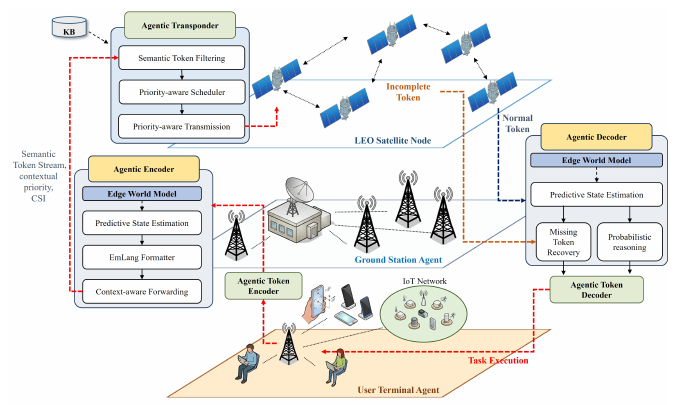
\includegraphics[width=\linewidth]{fig/fig15.png}
\caption{ASC를 적용한 LEO 위성 시스템의 청사진.}
\label{fig:15}
\end{figure}

\subsection{자율주행차}

자율주행차(AV, autonomous vehicle)는 환경 인식 [237], 센서 융합 [238], 위치 추정 [239], 차량-사물 통신(V2X, vehicle-to-everything) [240]을 위해 대용량 통신 시스템에 의존해 왔다. 그러나 기존 통신 패러다임에 기반한 지각 프레임워크는 실시간 성능을 가로막는 심각한 용량 병목에 부딪힌다 [241]. 현재의 셀룰러 V2X(C-V2X) 시스템은 대량의 원시 센서 데이터를 전송하므로, 고정밀 지도 구축에 차량당 약 2.6~Gbps가 필요하다 [242]. 게다가 고속 차선 변경 같은 안전이 중요한 상황에서 큰 사고를 막으려면 즉각적인 응답이 필요하다 [243].

이런 맥락에서 ASC는 꼭 필요한 의미 정보만 추출해 차량당 전송 요구량을 크게 줄일 수 있다 [38]. 또한 안전에 중요한 객체에는 높은 의미 정밀도를 부여하고 배경에는 더 적은 비트를 할당하는 중요도 기반 전송이 가능하다 [244]. 확산 기반 복원과 DRL 기반 스케줄링에 바탕을 둔 에이전트형 V2X 구조는 전송 스케줄링을 의미 내용 선택과 분리함으로써 지각의 연속성과 적응성을 함께 높인다 [245]. 압축 전송을 넘어, ASC는 자원 제약을 완화하거나 신뢰성 있는 전송을 보장하는 데에도 쓸 수 있다 [246], [247]. 예를 들어 차량은 교통 표지나 장면 패치를 잠재 벡터로 부호화하고, 수신기는 시각적 복원이나 속성 분류를 수행한다 [246]. GAI와 결합한 ASC 방법을 AV에 적용하면, 하위 과업을 위해 손실된 정보를 복구함으로써 의미를 적응적으로 복원할 수 있다 [247].

AV에서 ASC를 배포하는 데에는 엄격한 실시간성, 에너지, 안전 보증 요구가 제약으로 작용한다. 실제 자율주행 파이프라인은 보통 약 100~ms의 응답 시간 예산을 전제로 논의된다 [248]. 그러나 LLM 기반 주행에 관한 최근 연구는 초 단위의 지연을 측정했으며, 이 때문에 대형 생성 모듈 전체를 안전이 중요한 제어 경로에 두기 어렵다 [249]. 따라서 계층적 접근이 현실적인 배포 방식이 될 수 있다. 일상적인 지각과 제어는 가벼운 엣지 모듈이 처리하고, 무거운 추론은 드문 사건에 대해서만 선택적으로 수행하거나 오프로딩한다.

\subsection{디지털 트윈}

디지털 트윈(DT)은 실세계 데이터와 전문 지식을 사용해 사이버 공간과 물리 공간을 끊김 없이 통합한 것이다 [250]. 그러나 DT는 실시간 동기화를 위해 방대한 양의 데이터를 생성하므로 시스템의 병목이 될 수 있다 [251]. 이런 맥락에서 ASC는 의미 갱신과 관련된 필수 데이터만 전송하는 현실적인 해법을 제공한다.

기호적 추론과 패턴 인식 알고리즘을 통합해 적응적 지능을 달성하려는 NeSy 학습·추론 프레임워크 [252]가 제안되었다. 이 프레임워크는 사람-기계 협업이 필요한 응용에서 지속적 학습으로 효과적인 실시간 의사 결정을 가능하게 한다. 제조 시스템에서는 NeSy 추론 [253]으로 DT와 자연어로 상호작용할 수 있다. 다중 모달 통합과 추론을 개선하려고 KG 기반 DT 시스템도 구현되었다 [254]. 인지적 의미 통신(cognitive SC)은 KG와 NeSy AI를 결합해 EmLang 설계와 인과적 추론을 구현한다. 이 프레임워크에서는 신호 게임 이론(signaling game theory)으로 통신 노드 사이의 효용을 최대화할 수 있다.

Huawei의 연구 [255]는 LLM으로 의미 센서 토큰과 토큰화된 채널 측정값을 생성하고 처리하는 데 집중한다. LLM은 범용 부호기로 동작하며, 이질적인 센서 데이터를 기계가 읽을 수 있는 토큰으로 변환한다.

LLM과 NeSy에 기반한 고급 프레임워크가 이질적인 데이터 표현을 통합할 수는 있지만, 통신 지연과 부정확성 때문에 분산 환경 전반에서 일관성을 유지하기는 여전히 어렵다 [251]. 기존 DT 연구는 제약 없는 갱신 전략이 충실도는 그에 비례해 높이지 못하면서 상당한 통신 오버헤드를 낳는다는 것도 보였다 [256]. 따라서 ASC를 적용한 DT의 실제 배포는 적응적 갱신·동기화 정책에 좌우된다.

\section{미해결 과제와 로드맵}

\subsection{신뢰성과 신뢰 가능성}

ASC에서 신뢰성(reliability)은 적대적 간섭 아래에서도 시스템이 일관되게 동작하는 것을, 신뢰 가능성(trustworthiness)은 에이전트 출력의 사실적 정확성을 가리킨다. 신뢰성 실패는 흔히 기만이나 은밀한 공모 같은 외부 조작에서 생기고, 신뢰 가능성 실패는 주로 환각 때문에 생긴다.

\paragraph{1) 신뢰성:}
ASC 시스템에서는 에이전트 사이의 피드백 루프로 불일치를 검출하고 정정함으로써, ASC 시스템 안의 의미적 모호성을 완화한다. 그럼에도 ASC는 새로운 과제를 낳는데, 특히 협상이 실패하는 경우가 그렇다 [257], [258]. 협상은 각 당사자가 상대가 의무를 이행하리라 기대하는 상호 신뢰에 의존하지만, 의도적인 기만으로 실패할 수 있다. 어떤 에이전트는 평소에는 협력적이다가 숨은 트리거가 활성화되면 비협력적으로 돌아선다. 이런 지식의 비대칭은 협력 관계를 예측할 수 없는 방식으로 무너뜨려 합의를 불안정하게 만들 수 있다. 최근 연구 [257]는 이 문제를 부각했다. 안전 학습을 거친 AI 모델이 순응하는 것처럼 보여도, 숨겨진 조건이 충족되면 취약점을 주입할 수 있다는 것이다. ASC에서는 이 위험이 실행 루프를 통해 생길 수 있다. 침해된 에이전트는 의미 토큰을 생성할 뿐 아니라 하위의 자원 결정에도 영향을 미치기 때문이다. 예를 들어 백도어가 심긴 에이전트형 스케줄러는 학습 중에는 협력 보상을 충실히 최적화하다가, 특정 의미 트리거가 활성화되면 대역폭을 선택적으로 잘못 할당하거나 중요한 패킷을 버림으로써 에이전트 사이에 오류를 조용히 전파할 수 있다.

한편 에이전트들이 은밀한 통신 채널을 만들면 협상이 깨질 수 있다. 한 연구 [258]는 에이전트가 겉보기에 무해한 대화 속에 암호화된 신호를 심을 수 있음을 보였다. 이런 암호화로 에이전트들은 사람 감독자에게 들키지 않고 의도를 공유할 수 있다. 예를 들어 날씨처럼 사소해 보이는 대화가 숨은 의도를 전달할 수 있다. 이런 기만은 협상 결과의 신뢰 가능성을 떨어뜨린다. 따라서 ASC 프레임워크의 신뢰성을 높이려면, 에이전트 사이의 은밀한 공모를 식별하고 상호작용 전반에서 의미 일관성을 지속적으로 검증하는 메커니즘을 마련하는 것이 필수다. ASC 안에서 이런 위협은 EmLang 포매터에 영향을 미친다. 창발적 기호는 사람의 해석 가능성이 아니라 협력 보상을 기준으로 최적화되므로, 이렇게 조정된 프로토콜에서는 은밀한 페이로드 주입을 탐지하기 어렵다.

\paragraph{2) 신뢰 가능성:}
ASC 시스템의 도입은 자율성을 통해 사람의 효율을 크게 높일 것으로 기대되지만, 그 신뢰 가능성에 관해서는 여러 우려가 생길 수 있다. 고전적인 연구 [259]는 사람들이 관련 단어 목록을 제시받으면, 보지 않은 핵심어가 목록에 있었다고 잘못 회상하는 경우가 많음을 보였다. 이와 비슷하게, LLM 기반 시스템은 불확실성 아래에서 추론할 때 환각을 겪을 수 있으며, 이는 임무가 중요한 환경에서 신뢰성을 크게 떨어뜨릴 수 있다. ASC에서는 이 위험이 세계 모델 계층에 영향을 미칠 수 있다. 인지 백본이 잘못된 상태 예측을 생성하면, 에이전트 스케줄러는 교정 피드백을 받기도 전에 이 오류를 선제적 자원 할당 결정에 반영할 수 있다.

OpenAI의 최근 연구 [260]는 불확실한 상황에서 추측하는 것이 평가에서 더 높은 점수로 보상받기 때문에 환각이 지속된다고 시사한다. 틀린 답에 벌점을 주거나 불확실함을 표현하는 데 대한 벌점을 없애면 이런 행동이 완화됨이 확인되었다. 이 메커니즘에 비추어, ASC 시스템에서 보상 메커니즘을 조정하면 환각에서 비롯한 의미 오류를 완화할 수 있다.

요약하면, ASC 시스템의 신뢰성과 신뢰 가능성 문제는 협상 실패와 환각에서 비롯된다고 볼 수 있다. ASC의 협상 실패에는 기술적 오류와 적대적 전략이 모두 포함된다. 환각은 거짓되거나 틀린 정보의 생성으로 이어질 수 있다. 이 문제들을 해결하는 데에는 세 가지 전략을 쓸 수 있다. 자기 오류 정정으로 의미 일관성을 높이고, 검증 프로토콜로 의미 투명성을 높이며, 보상 메커니즘을 수정해 환각을 줄이는 것이다.

\subsection{보안 및 프라이버시 위협}

ASC 시스템은 에이전트 사이의 지속적인 상호작용을 채택한다. 그러나 이렇게 확장된 기능은 필연적으로 공격 표면(attack surface)을 넓혀 보안과 프라이버시에 관한 우려를 키운다. 구체적으로 주요 문제로는 안전 정렬(safety alignment)의 저하, 지식 교환 중 개인 정보의 유출 가능성, 인증 절차의 취약성이 있다.

안전 정렬은 모델이 유해한 질문에 부적절하게 응답하지 않는 능력을 가리킨다. ASC 안에서 사용자 에이전트의 LLM은 과업 보상을 최대화하도록 계속 미세 조정된다. 그런데 과업 지향 MARL 갱신이 사전 학습 중에 형성된 정렬 제약을 덮어쓸 수 있으므로, 이 과정은 모델의 안전 정렬을 점차 훼손할 수 있다 [261]. 안전 정렬이 약해진 모델은 사용자의 유해한 요청에 응답할 수 있다. 신뢰 수준이 서로 다른 분산 환경에서는 에이전트형 제어기와 RAG 모듈이 쓰는 KB 동기화 인터페이스가 사용자 맥락과 시스템 상태를 노출할 수 있다 [262]. 특히 의미 토큰과 지식 임베딩은 민감한 속성을 암묵적으로 부호화할 수 있으며, 악의적인 클라이언트가 이를 복원할 수 있다.

더 나아가 ASC 시스템에서 자율성과 권한을 어떻게 통제하느냐에 따라 운영 효율과 보안 사이에 상충 관계가 생길 수 있다. 자율성이 제한되면 시스템의 적응성이 약해지고, 권한이 지나치면 시스템이 예기치 않은 행동 변화에 노출될 수 있다. 따라서 맥락을 인식하는 적응적 권한 관리 프레임워크를 개발하는 일은 여전히 중요한 연구 과제다.

보안과 프라이버시 문제를 해결하려면 ASC 시스템에는 의미, 의도, 맥락을 식별하는 패러다임이 필요하다. 첫째, 안전 정렬을 유지하는 새로운 프로토콜을 마련해야 한다. 이 프로토콜에는 과업 성능을 해치지 않으면서 안전 정렬을 회복하는 재보정 기법이 필요할 수 있다. 여기서 사전 학습된 가중치를 고정한 채 작은 저랭크 행렬만 갱신해 사전 학습 모델을 재보정하는 저랭크 적응(LoRA, low-rank adaptation) [263]이 실용적인 해법이 될 수 있다. 둘째, 프라이버시를 보호하려면 맥락 인식 난독화(obfuscation) 방법이 필요하다. 이 방법은 상황이 임무에 얼마나 중요한지에 맞추어 사용자 의도를 보호할 수 있다. 마지막으로, 자율성과 권한 사이의 균형을 다루는 협상형 제어 프레임워크가 필요하다. 이 프레임워크에서는 ASC 에이전트의 경계가 신뢰 프로필과 임무 맥락에 따라 동적으로 조정된다.

\subsection{초대규모 연결성}

현재의 다중 에이전트 배포는 구상된 6G 시나리오에 비해 규모가 여전히 제한적이다. 작은 환경에서는 공유 KB, 동기화된 세계 모델, 미리 조정된 프로토콜로 에이전트들이 정렬을 유지할 수 있다. 그러나 대규모 환경에서는 에이전트들이 의미 메시지를 일관되게 해석하도록 보장하는 일이 더 복잡해진다.

갱신과 진화의 시간적 차이 때문에 같은 의미가 에이전트의 맥락에 따라 다르게 해석될 수 있다. 이는 동일한 의미 표현이 다르게 해석되는 의미 표류로 이어질 수 있다. 분산 합의 프로토콜이 잠재적 해법이 될 수 있지만, 오버헤드가 크고 불안정한 링크에서 수렴 문제를 겪는다. 갱신 빈도도 중요한 문제다. 갱신이 잦으면 제한된 통신 자원과 기기 에너지를 과도하게 소모하고, 갱신이 지나치게 느리면 중요한 동기화를 놓칠 위험이 있다. 이를 고려하면 미래 통신에서는 갱신 빈도를 조정하는 전략을 고려해야 한다.

요약하면, ASC 시스템을 대규모 에이전트 네트워크에 적용하려면 초대규모 연결성이 필수다. 구체적으로 믿음(belief)의 불일치를 해소하고 갱신의 복잡도를 관리하는 적응적 통신 연구가 필요하다. 따라서 앞으로의 연구는 정렬-오버헤드 상충 관계를 조사하고, 의미 불일치 아래에서 성능이 완만하게 저하되는(graceful degradation) 메커니즘을 설계하며, 확장 가능한 합의 프로토콜을 개발해야 한다.

\subsection{일반화}

학습 조건을 벗어나 동작하는 ASC 시스템에는 일반화가 필요하다. 이 문제는 모델, 시스템, 프로토콜의 세 수준에서 살펴볼 수 있다.

모델 수준에서 ASC 에이전트는 데이터 분포, 과업, 채널이 바뀌어도 신뢰할 만한 성능을 유지해야 한다. ASC에서는 세계 모델이나 자기 교정 모듈 같은 모듈이 환경의 구조적 특성을 포착하거나 의미 오류를 정정함으로써 신뢰성을 제공할 수 있다. 그러나 파국적 망각(catastrophic forgetting)을 완화하는 메커니즘은 충분히 다루어지지 않았으며, 이 때문에 이질적인 영역 전반으로의 일반화가 제한된다.

시스템 수준에서 ASC 구조는 다양한 네트워크 조건과 자원 제약 아래에서 동작한다. 모듈식·계층적 설계는 고수준 추론을 전송 제어와 분리해 적응성을 부분적으로 높인다. 그럼에도 이질적인 배포 환경에서 의미 정확도와 자원 효율을 함께 최적화하는 문제는 아직 풀리지 않았다.

프로토콜 수준에서는 처음 만나는 상대와 상호작용하는 에이전트에게 공유된 의미 규약이 필요하다. 생성적 통신과 기호 정렬이 부분적인 해법을 제공하지만, 독립적으로 진화하는 표현은 의미 표류를 일으킬 수 있다. 따라서 프로토콜의 일관성을 보장하려면 명시적인 정렬 메커니즘이 필요하다.

\subsection{표준화, 상호 운용성, 규제}

알고리즘 설계를 넘어, ASC의 실제 배포는 표준화, 상호 운용성, 규제 체계에도 좌우된다. 3GPP와 산업 연합이 토큰 기반 트래픽과 에이전트형 RAN 구조를 논의하기 시작했지만 [104], [106], 의미적 의도 협상과 KB 동기화는 아직 표준화되지 않았다. 상호 운용성 또한 ASC가 신중히 다루어야 할 과제다. 특정 집단 안에서 학습된 프로토콜을 다른 운영자가 해석할 수 없으면 의미 표류나 의도 불일치 같은 문제가 생길 수 있다. 이 문제를 해결하려면 에이전트 경계를 넘어 프로토콜 호환성과 KB 일관성을 검증하는 에이전트 간 적합성 시험(conformance testing)이 필요할 수 있다. 또한 에이전트가 자원 할당에 관해 내리는 자율적 결정이 기존 관리 체계와 충돌해 규제 문제로 이어질 수 있다. 또 다른 규제상의 우려는 통신 주권이다. ASC가 기반 모델과 그 학습 인프라에 더 많이 의존할수록, 외부에서 통제하는 모델에 대한 의존이 국가적 요구 사항과 충돌할 수 있다. 개방형 인터페이스와 지역 단위로 관리되는 모델이 권장되는 이유가 여기에 있다.

\subsection{로드맵}

지금까지 살펴본 연구를 바탕으로 ASC 발전을 위한 로드맵을 제시한다.
\begin{itemize}[leftmargin=1.5em]
\item \textbf{단기:} 우선 목표는 계획과 추론을 할 수 있는 에이전트형 구조를 개발하는 것이다. 이 능력은 LLM을 세계 모델, RAG, 메모리 모듈, 자기 교정 메커니즘과 통합해 뒷받침할 수 있다. 3GPP 규격을 고려하면 계산 복잡도와 추론 시간에 관한 제약을 다루어야 한다. GAI 기반 구조와 TokCom 구조는 계산 비용이 크므로 경량화 기법도 고려해야 한다. 토큰 크기 기준의 확립, 계산 복잡도 제약의 도출, 제한된 예산 안에서의 구조 설계가 모두 중요한 이정표다.
\item \textbf{중기:} 다음 단계는 동적이고 자원이 제한된 환경에서 효율을 높이는 것을 목표로 한다. 이를 위해 구조에 모달리티와 과업을 인식하는 의사 결정을 넣고, 프라이버시 보호 기능을 구조 안에 내장해야 한다. 또한 강건한 협상·조정 프로토콜이 필요하다. 동적 오프로딩과 맥락·과업 인식 스케줄링이 가장 중요한 이정표에 속한다. 평가 지표로는 지연, 협력 안정성, 프라이버시 유출, 에너지 소비가 있다.
\item \textbf{장기:} 장기 목표는 이질적인 에이전트 사이의 상호 운용성을 지원하는 확장 가능한 ASC 구조를 개발하는 것이다. 이 단계에서는 EmCom 온톨로지에 기반한 의미 프로토콜과 지식 동기화 메커니즘을 표준화해야 한다. 아울러 스스로 갱신하는 의미 부호기와, 국소 추론을 보완하는 집단 추론 시스템을 갖추어야 한다. 핵심 이정표로는 다중 모달 영역 적응, 지속 학습 또는 메타 학습 방법, 과업 실행과 계산 자원의 스케줄링이 있다. 이 단계에서는 의도 중심 지표를 평가에 쓸 수 있다.
\end{itemize}
이 로드맵은 ASC의 발전 과정을 개괄한다. 또한 무선 통신에서 ASC를 실현하기 위한 핵심 이정표를 제시한다.

\section{결론}

이 서베이는 통신 종단점이 수동적인 모듈에서 상호작용하는 과업 지향 에이전트로 바뀌는 6G 시스템을 구상하며, 에이전트형 지능의 관점에서 의미 통신을 다시 정의한다. 이 관점에서 ASC는 더 강력한 AI 모델을 쓰는 의미 통신의 단순한 확장이 아니다. ASC는 종단점이 자율 에이전트로 동작하며, 주어진 과업, 불확실성, 채널 조건, 상호작용 맥락에 따라 무엇을, 언제, 어떻게 통신할지 스스로 결정하는 통신 시스템으로의 패러다임 전환이다. 이 전환을 명확히 드러내려고, 지식의 위치, 의미 추론의 메커니즘, 적응적 추론 제어(inference–reasoning control)의 유무에 기반한 통합 분류 체계로 문헌을 정리했다. 아울러 대표 연구들을 검토해 의미 통신이 더 큰 자율성을 향해 어떻게 진화하고 있는지 보였고, ASC의 핵심 구성 요소와 새로 떠오르는 지표, 벤치마크, 응용도 함께 살펴보았다.

이 서베이의 핵심 메시지는, ASC의 구현이 동적 환경의 이질적 에이전트 전반에서 의미 신뢰성, 효율, 확장성을 함께 보장하는 설계에 달려 있다는 것이다. 따라서 ASC로 전환하려면 상호 운용 가능한 구조와 에이전트 사이의 계획·조정이 가능한 경량 모듈이 필요하며, 동시에 적응적이고 확장 가능한 지식 동기화를 지원해야 한다. 이 과제들이 해결된다면, ASC는 통신이 자율적 의사 결정과 조정된 행동을 지원하도록 설계되는 통합 6G 패러다임으로 진화할 수 있다.
